% mnras_template.tex 
%
% LaTeX template for creating an MNRAS paper
%
% v3.0 released 14 May 2015
% (version numbers match those of mnras.cls)
%
% Copyright (C) Royal Astronomical Society 2015
% Authors:
% Keith T. Smith (Royal Astronomical Society)

% Change log
%
% v3.0 May 2015
%    Renamed to match the new package name
%    Version number matches mnras.cls
%    A few minor tweaks to wording
% v1.0 September 2013
%    Beta testing only - never publicly released
%    First version: a simple (ish) template for creating an MNRAS paper

%%%%%%%%%%%%%%%%%%%%%%%%%%%%%%%%%%%%%%%%%%%%%%%%%%
% Basic setup. Most papers should leave these options alone.
\documentclass[fleqn,usenatbib]{mnras}

% for error: too many math alphabets used in version normal
\newcommand\hmmax{0}
\newcommand\bmmax{0}

% MNRAS is set in Times font. If you don't have this installed (most LaTeX
% installations will be fine) or prefer the old Computer Modern fonts, comment
% out the following line
\usepackage{newtxtext,newtxmath}
% Depending on your LaTeX fonts installation, you might get better results with one of these:
%\usepackage{mathptmx}
%\usepackage{txfonts}

% Use vector fonts, so it zooms properly in on-screen viewing software
% Don't change these lines unless you know what you are doing
\usepackage[T1]{fontenc}
\usepackage{ae,aecompl}


%%%%% AUTHORS - PLACE YOUR OWN PACKAGES HERE %%%%%

% Only include extra packages if you really need them. Common packages are:
\usepackage{graphicx}	% Including figure files
\usepackage{amsmath}	% Advanced maths commands
\usepackage{amssymb}	% Extra maths symbols
\usepackage{hyperref}
\usepackage{multirow}
\usepackage{tabularx}
\usepackage[group-separator={,}]{siunitx}
\usepackage{bm}
\usepackage{xcolor}

%%%%%%%%%%%%%%%%%%%%%%%%%%%%%%%%%%%%%%%%%%%%%%%%%%

%%%%% AUTHORS - PLACE YOUR OWN COMMANDS HERE %%%%%

% Please keep new commands to a minimum, and use \newcommand not \def to avoid
% overwriting existing commands. Example:
%\newcommand{\pcm}{\,cm$^{-2}$}	% per cm-squared
\newcommand{\R}{\color{red}}

%%%%%%%%%%%%%%%%%%%%%%%%%%%%%%%%%%%%%%%%%%%%%%%%%%

%%%%%%%%%%%%%%%%%%% TITLE PAGE %%%%%%%%%%%%%%%%%%%

% Title of the paper, and the short title which is used in the headers.
% Keep the title short and informative.
\title[Cosmic shear analysis]{Progress report: cosmic shear analysis for red/blue source galaxies}

% The list of authors, and the short list which is used in the headers.
% If you need two or more lines of authors, add an extra line using \newauthor
\author[S.-S. Li]{
Shun-Sheng Li,$^{1}$\thanks{E-mail: ssli@strw.leidenuniv.nl}
\\
% List of institutions
$^{1}$Leiden Observatory, Leiden University, P.O. Box 9513, 2300 RA Leiden, the Netherlands\\
}

% These dates will be filled out by the publisher
\date{Accepted XXX. Received YYY; in original form ZZZ}

% Enter the current year, for the copyright statements etc.
\pubyear{2019}

% Don't change these lines
\begin{document}
\label{firstpage}
\pagerange{\pageref{firstpage}--\pageref{lastpage}}
\maketitle

% Abstract of the paper
\begin{abstract}
This is a report for the progress of the project: Cosmic shear analysis using red/blue split of source galaxies: systematic effects and intrinsic alignments.
\end{abstract}

% Select between one and six entries from the list of approved keywords.
% Don't make up new ones.
\begin{keywords}
gravitational lensing: weak -- cosmology: observations
\end{keywords}

%%%%%%%%%%%%%%%%%%%%%%%%%%%%%%%%%%%%%%%%%%%%%%%%%%

%%%%%%%%%%%%%%%%% BODY OF PAPER %%%%%%%%%%%%%%%%%%

\section{Reproduce Hildebrandt et al. 2018}
This section is about the reproduction of work by \citet{2018arXiv181206076H}. The goal of this part of work is to test the algorithm performance and build a well-tested pipeline for the further cosmic shear analysis involving red/blue samples.

\subsection{Data}
The combined KiDS+VIKING-450 (KV450) shear catalogues~\citep{2018arXiv181206077W} are obtained from the KiDS website~\footnote{\url{http://kids.strw.leidenuniv.nl/DR3/kv450data.php}}. The downloaded catalogues contain only `good' sources and the `$3\times 4\times 4$' grid. The `$3\times 4\times 4$' flag denotes the division scenario of the whole KV450 catalogue based on PSF size and the complex ellipticity. These sub-catalogues are recalibrated with specific weight to account for the uncertainty in the ellipticity measurement. 

According to the description made at the website, the only selection criterion one has to apply before using the catalogues is ``GAAP\_Flag\_ugriZYJHKs $==0$''. However, we here note that this mask is not sufficient to remove all the ``bad'' data in terms of magnitude measurement, such as those with magnitudes equal $99$ or $-99$. Hence we set a new criterion to remove all these ``outliers''. Also applied is a cut in r-band magnitude with $20<m_r<25$ ({\R why?}). The total number of objects after applying all these selections (\num{9181855}) is roughly $30\%$ lower than that from the naive ``GAAP\_Flag\_ugriZYJHKs $==0$'' mask (\num{13241807}). Detailed information about object numbers can be found in Table~\ref{table:si}.

Next, we calculate the correlation function based on these two data sets and compare it with the published result from \citet{2018arXiv181206076H}.

\subsection{Correlation Function}
The 2-point shear correlation function is calculated based on five tomographic bins. These bins are built according to the sources' nine-band-photometry redshifts estimated using the BPZ (Bayesian Photometric Redshift) photo-$z$ code~\citep{BPZ_2000ApJ,BPZ_2006AJ} with an improved redshift prior from \citet{BPZ_2014ApJ}. Following \citet{2018arXiv181206076H}, the five bins are determined with redshift ranges $0.1<z_B\leq 0.3$, $0.3<z_B\leq 0.5$, $0.5<z_B\leq 0.7$, $0.7<z_B\leq 0.9$, $0.9<z_B\leq 1.2$. The corresponding source numbers are summarized in Table~\ref{table:si}.

By using the public TREECORR code~\citep{TREECORR_2004MNRAS}, the correlation function between bins $i$ and $j$ can be measured with
\begin{equation}
\label{equ:CF}
    \xi^{ij}_{\pm}(\theta)=\frac{\sum_{ab}w_aw_b\left[\epsilon_t^i(\bm{x}_a)\epsilon_t^j(\bm{y}_b)\pm\epsilon_{\times}^i(\bm{x}_a)\epsilon_{\times}^j(\bm{y}_b)\right]}{\sum_{ab}w_aw_b}~,
\end{equation}
where $\epsilon_{t,\times}$ are the tangential and cross ellipticities with respect to the vector $\bm{x}_a-\bm{y}_b$ between a pair of galaxies $(a,b)$, $w$ is a weight reported from the shape measurement using the {\it lens}fit algorithm \citep{lensfit_2007MNRAS.382..315M,lensfit_2008MNRAS.390..149K,lensfit_2013MNRAS.429.2858M}. The column we used for this weight is named as ``recal\_weight'' in the downloaded catalogues.

The Sums shown in equation~(\ref{equ:CF}) go over all galaxy pairs in an interval $\Delta\theta$ around $\theta$, which requires a settlement of spatial bins. As in \citet{2018arXiv181206076H}, we define nine logarithmically spaced bins within $[0.5', 300']$ and use the first seven bins for $\xi_{+}$ and the last six for $\xi_{-}$. The reason behind these choices is detailed in \citet{2018arXiv181206076H}. Accordingly, the estimation of correlation function yields $(7+6)\times 15=195$ points, which build the KV450 cosmic shear data vector. Our reproduced results along with the results from \citet{2018arXiv181206076H} are shown in Figs.~(\ref{fig:xip}) and (\ref{fig:xim}).

\newpage

One thing worthy of note is the shear biases, which mainly result from the uncertainty associated with the shape measurement process. These biases are normally determined using image simulations~\citep{ImSim_2017MNRAS.467.1627F,ImSim_2019A&A...624A..92K}. As detailed in the section 4 of \citet{2018arXiv181206076H}, the shear bias can be quantified using linear parametrisation~\citep{shearbias_2006MNRAS.368.1323H,shearbias_2007MNRAS.376...13M},

\begin{equation}
\label{equ:shearbias}
g^{\rm obs}_i = (1+m_i)g^{\rm true}_i + c_i~,
\end{equation}
where $g^{\rm obs}_i$ and $g^{\rm true}_i$ are the observed and true reduced gravitational shears, respectively, with $i=1,2$ refers to the two different components.

The two type of biases $m_i$ and $c_i$, usually referred to as the multiplicative bias and the additive bias, respectively, have different sources and properties, therefore, require different treatments. Thanks to the sophisticated image simulations performed in \citet{ImSim_2019A&A...624A..92K}, the multiplicative bias in the KV450 catalogue is solidly quantified and calibrated. Nevertheless, the treatment of the additive bias (also known as the c-term) is much more uncertain. Without a full model, the c-term is usually accounted for with a purely emprical approach. That is to first estimate the value for c-term per tomographic bin by estimating the weighted average of the measured galaxy ellipticities $\epsilon_{1,2}$, then calibrate the ellipticities by subtracting this c-term before being passed to the shear correlation function calculations. ({\R Not confident about this paragraph's explanation.})

We are not sure if the c-term is corrected in the downloaded catalogues. So we calculated the c-term using the strategy mentioned above, and the results are presented in Table~\ref{table:si}. ({\R why several negative values in c-term?}) The columns we used are ``bias\_corrected\_e1'', ``bias\_corrected\_e2'', ``recal\_weight'', and the specific realization is learned from the ``KiDS-VIKING\_pipeline''. The trick is, instead of directly averaging all the samples in each bin, they first generate 30 sets of random samples from the original data with the same size and calculate the weighted mean for each set. The final result is then obtained by averaging these 30 means. This treatment provides us an error for the c-term estimation, which is just the standard deviation of the 30 means. 

Given above concern, our final results (Figs.~\ref{fig:xip} for $\xi_+$ and \ref{fig:xim} for $\xi_-$) contain four different sets. They are naively selected data set (``GAAP\_Flag\_ugriZYJHKs $==0$'') with new estimated c-term subtracted and without c-term subtraction (marked as ``{\it pre} with c-term'' and ``{\it pre} without c-term'', respectively in the figures), and magnitude selected data set with and without new estimated c-term substracted (marked as ``{\it new} with c-term'' and ``{\it new} without c-term'', respectively). As can be seen, the treatment of c-term does not bring much difference. This is consistent with the statement made by \citet{2018arXiv181206076H} that the additive biases are generally small and does not have any significant effect on the measurements. ({\R Or means that the c-term is already corrected in the downloaded catalogues?}) One the other side, the magnitude selection of the data does introduce notable difference in the final result, especially for bins ``1-1'' and ``1-5''. This difference cautions us about the proper treatment of the data selection. The minor discrepancy between our reproduced result and the \citet{2018arXiv181206076H} result also requires further discussion. Given the trivial influence from the bias calibration, this kind of discrepancy is most likely also rendered from the data selection procedure.

\subsection{Cosmic Shear Signal}

\section{Red/Blue Split of Source Galaxies}
This section discusses the selection and properties of red/blue samples. The goal of this part of work is to build the red/blue samples for the cosmic shear analysis.

\subsection{Selection}

\subsection{Properties}

\section{Cosmic Shear Analysis for Red/Blue Samples}
This is the main course.


\begin{table*}
\caption{Source information in the five tomographic redshift bins. ``{\it pre}'' and ``{new}'' refer to data selections without and with magnitude cut, respectively. ({\R why several negative values in c-term?})}
\label{table:si}
\begin{tabularx}{\textwidth}{c|c|rr|rrrr}
% ---------------------------------------------------------------------------
\hline
\hline
Bin & $z_B$ range &  \multicolumn{2}{c|}{Number} & \multicolumn{4}{c}{c-term $(\times 10^{-4})$} \\
 & & {\it pre} & {\it new} & \multicolumn{2}{c}{\it pre} & \multicolumn{2}{c}{\it new} \\
 & & & & $\epsilon_1$ & $\epsilon_2$ & $\epsilon_1$ & $\epsilon_2$ \\
\hline
% ----------------------------------------------------------------------------------------------------------------------------------------------------
1 & $(0.1, 0.3]$ & \num{1027504} & \num{958244} & $3.0\pm 3.1$ & $6.8\pm 2.4$ & $-8.9\pm 2.5$ & $6.0\pm 2.3$ \\
2 & $(0.3, 0.5]$ & \num{1798830} & \num{1394353} & $3.7\pm 1.5$ & $6.2\pm 1.9$ & $4.1\pm 2.3$ & $6.2\pm 2.7$ \\
3 & $(0.5, 0.7]$ & \num{3638808} & \num{2424461} & $7.7\pm 2.1$ & $3.6\pm 2.0$ & $4.0\pm 1.8$ & $5.7\pm 1.9$ \\
4 & $(0.7, 0.9]$ & \num{2487124} & \num{1617429} & $1.9\pm 2.1$ & $1.0\pm 1.7$ & $5.0\pm 2.1$ & $2.3\pm 2.0$ \\
5 & $(0.9, 1.2]$ & \num{2781676} & \num{1802022} & $-10\pm 1.9$ & $7.5\pm 1.8$ & $1.6\pm 2.2$ & $0.6\pm 2.9$ \\
\hline
all bins & $(0.1, 1.2]$ & \num{11733942} & \num{8196509} & - & - & - & - \\
all & ($-\infty$, $\infty$) & \num{13241807} & \num{9181855} & - & - & - & - \\

% ----------------------------------------------------------------------------------------------------------------------------------------------------
\hline
\end{tabularx}
\end{table*}

\begin{figure*}
    \centering
    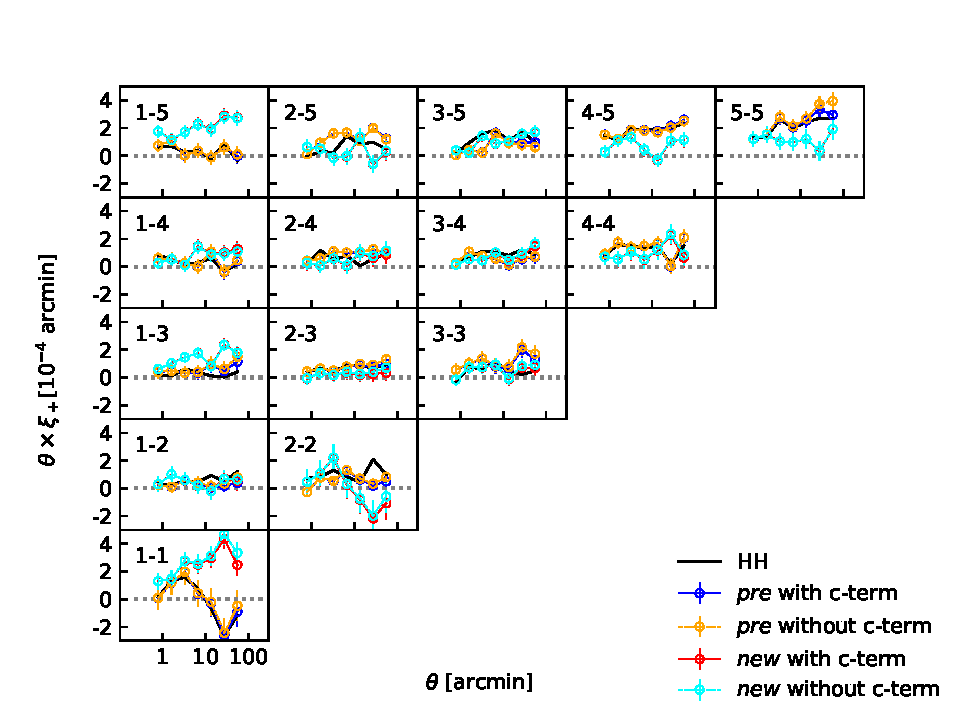
\includegraphics{compare_xip.pdf}
    \caption{Correlation function $\xi_+$ plotted as $\theta\times\xi_+$. ``HH'' refers to the result from \citet{2018arXiv181206076H}. The four results from our reproduction are refered to as ``{\it pre} with c-term'', ``{\it pre} without c-term'' for ``GAAP\_Flag\_ugriZYJHKs $==0$'' selected data with and without c-term subtraction, ``{\it new} with c-term'', ``{\it new} without c-term'' for magnitude selected data with and without c-term subtraction. The errors shown are reported by the TREECORR code, which are different from the errors shown in \citet{2018arXiv181206076H} who used the square root of the diagonal of the analytical covariance matrix. }
    \label{fig:xip}
\end{figure*}

\begin{figure*}
    \centering
    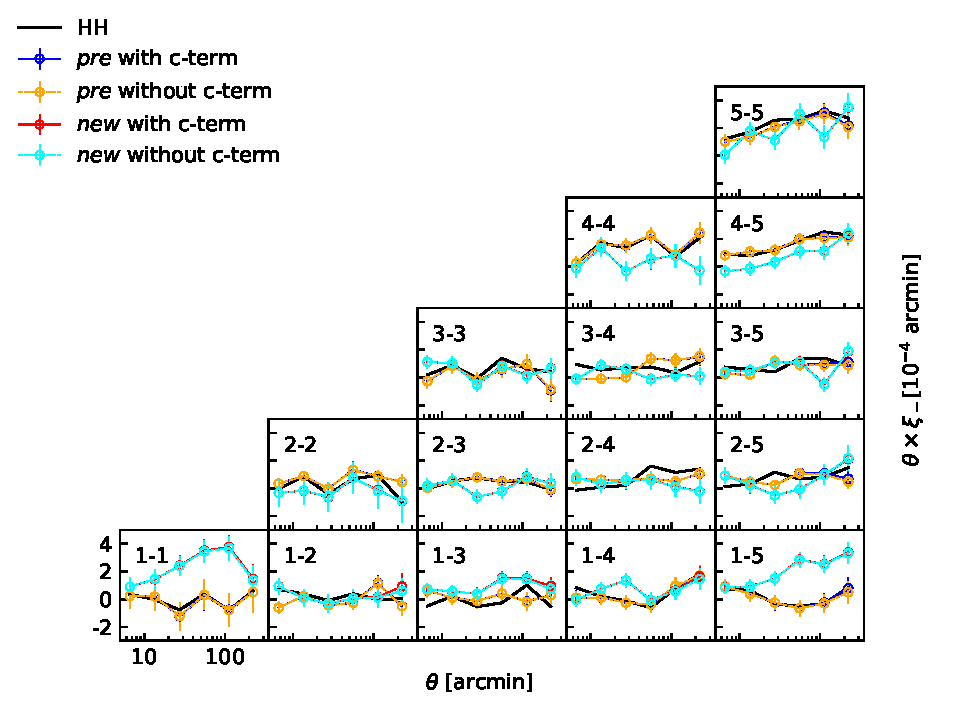
\includegraphics{compare_xim.pdf}
    \caption{Correlation function $\xi_-$ plotted as $\theta\times\xi_-$. ``HH'' refers to the result from \citet{2018arXiv181206076H}. The four results from our reproduction are refered to as ``{\it pre} with c-term'', ``{\it pre} without c-term'' for ``GAAP\_Flag\_ugriZYJHKs $==0$'' selected data with and without c-term subtraction, ``{\it new} with c-term'', ``{\it new} without c-term'' for magnitude selected data with and without c-term subtraction. The errors shown are reported by the TREECORR code, which are different from the errors shown in \citet{2018arXiv181206076H} who used the square root of the diagonal of the analytical covariance matrix. }    \label{fig:xim}
\end{figure*}


% \section*{Acknowledgements}

% The Acknowledgements section is not numbered. Here you can thank helpful
% colleagues, acknowledge funding agencies, telescopes and facilities used etc.
% Try to keep it short.

%%%%%%%%%%%%%%%%%%%%%%%%%%%%%%%%%%%%%%%%%%%%%%%%%%

%%%%%%%%%%%%%%%%%%%% REFERENCES %%%%%%%%%%%%%%%%%%

% The best way to enter references is to use BibTeX:

\bibliographystyle{mnras}
\bibliography{reference} % if your bibtex file is called example.bib

%%%%%%%%%%%%%%%%%%%%%%%%%%%%%%%%%%%%%%%%%%%%%%%%%%

%%%%%%%%%%%%%%%%% APPENDICES %%%%%%%%%%%%%%%%%%%%%

% \appendix

% \section{Some extra material}

% If you want to present additional material which would interrupt the flow of the main paper,
% it can be placed in an Appendix which appears after the list of references.

%%%%%%%%%%%%%%%%%%%%%%%%%%%%%%%%%%%%%%%%%%%%%%%%%%


% Don't change these lines
\bsp	% typesetting comment
\label{lastpage}
\end{document}

% End of mnras_template.tex